\chapter{Book III: the late work, and the lists in front of it}

\section{A book with its lists at the front}

Book III is the last of the work books and the one that runs to the painter's death. It has a printed alphabetical thumb index cut into its fore-edge, and she used the tabs to file the lists: Prizes under \q{G H}, Reproductions under \q{M Mc}, Gifts under \q{V}, Whereabouts under \q{C D}, each with the Book I page number beside it because each list continues one begun there (index, ref 18022). Nineteen unnumbered sheets of these lists stand in front of the work book; then the oils on the odd leaves from 1 to 89, Hotel Lobby to The Two Comedians; then the watercolours from Mexico, Wyoming and the Cape on leaves 101 to 125; and at the back two more Whereabouts leaves, a Frames memorandum and five leaves of Memoranda, which are continuous prose and the densest writing in the volume.

The title page announces the dealer, and gets his death wrong: \q{Frank K. M. Rehn sole dealer since Oct. 1924. The Rehn Gallery 683 - 5th Ave. N.Y.C. In summer of 1960, moved to 36 East 61st St. John J. \unc{Chaney} succeeding Frank K. M. Rehn as Sole director, Since 1953. Frank K. M. Rehn died in 1958 thru stroke \& long illness since summer 1953.} (title, ref 16528). The Memoranda leaf at the back has him \q{stricken Early Sept. 1953} and \q{Died there Early in 1956}, and Book II has March 1956. The 8 on the title page is written over another figure. She corrected the record, but not everywhere, and the edition lets each leaf say what it says.

\section{The pictures, and what she said they were}

The descriptive habit of Book II continues, and it changes. There are still colour plots: Hotel Lobby, \q{Girl beautiful blond, dull blue dress, flesh colored stockings. Older woman, white hair, coral silk dress, black coat + hat.} (\lf{Book III}{1}{16279}); Summer Time, \q{Big strong girl in thin white dress, flesh showing thru of right upper leg. \ldots\ Otherwise entire absence of local color as such.} (\lf{Book III}{3}{17456}). There are still names: Deborah and Sammy in Conference at Night (\q{Deborah is blond, a queen in her own right. \ldots\ Sammy better looking than here in drawing.}, \lf{Book III}{29}{17590}); Sheila and Adam in Sea Watchers (\q{Irish girl, gentle, sweet, large - Yankee clam digger - very fine people - on New England coast for late swim. Inventions of E.H.}, \lf{Book III}{47}{18177}); Dinah in South Carolina Morning; Toots in Second Story Sunlight, \q{good Toots, alert but not obstreperous. lamb in wolf's clothing}, with the marginal \q{the painter quoted} (\lf{Book III}{73}{17872}); Nora in Intermission, \q{E. H. says she is “Nora”. \ldots\ E. says Nora is on the way of becoming an “egg head”! An efficient secretary or prized chatelaine of big house.} (\lf{Book III}{81}{17386}). \q{Inventions of E.H.}, \q{the painter quoted}, \q{E. H. says}: here, for once, the names are attributed to him, and it is worth noticing that she takes the trouble to say so, as if she knew that a reader might assume they were hers.

But the descriptions in Book III are shorter, and they are more willing to say what a picture is \emph{about}. Summer Evening, entire: \q{She standing out for matrimony.} (\lf{Book III}{25}{18128}). Sun in an Empty Room, entire: \q{green bushes outside window. White light + uncompromising shadows. Stark.} (\lf{Book III}{83}{17402}). Hotel by a Railroad: \q{Emphasis on mood. Wife bitterly watches husband + tracks below window.} (\lf{Book III}{45}{17302}), which the transcriber rightly calls the only place in its batch where she says what a picture is about rather than what colour it is. Two Puritans: \q{2 white houses (dull Oct. day) loom like white petunias. Wan whiteish sky.} and \q{The halo of a pale blond beauty about this one. In class with Solitude, Rooms by the Sea, Moonlight Interior.} (\lf{Book III}{15}{16329}). October on Cape Cod carries the nearest thing in the archive to a statement of the painter's mind, and she marks it off the record: \q{“Peace, quiet, no birds sing.” “Some day you will be quiet too” - E. H.'s favorite Goethe. (strictly off the record)} (\lf{Book III}{19}{16838}).

Rooms by the Sea has an alias in its title line, \q{Alias “The Jumping Off Place”}, and a defence: \q{Inside contrasts not planned for intentional dramatic effect but as observed in a room full of light on Cape Cod \ldots\ Nothing of the palatial tourist camp. “Jumping Off Place” for name, turned down - but moonlight overtones ascribed by some.} (\lf{Book III}{41}{18347}). Hotel Window, of 1955, answers a critic nobody has named: \q{What ever interests woman gazing out must occur off stage at left of canvas \ldots\ Picture definitely not called: “Alone in the City at night.” But why not?} (\lf{Book III}{55}{16671}). Sunlight in a Cafeteria: \q{Sunlight + Space the whole story, the 2 figures quite negated by light on walls of large forms used. \ldots\ She a voluptuous blond. \ldots\ “Eating not interested in Color!”} and, of the buyer, \q{He saw this canvas in studio, having climbed up the 74 steps of 3 Washington Square North for that purpose.} (\lf{Book III}{65}{17966}). Excursion into Philosophy: \q{Real Hopper landscape out of window: A.M. Sun in blue sky touching green dune tops \ldots\ the open book is Plato, reread too late. \ldots\ Painted in 11 days. Aug 15'' - 26'', 1959.} (\lf{Book III}{69}{18472}). \q{Real Hopper landscape}: she has begun to write about him as a public figure, and a picture is now a Hopper.

Her verdicts on frames, hangings and museums sharpen with age. A Woman in the Sun: \q{Tragic figure of small woman, blond, straight brown hair, grabs cigarette before shimmy shirt. \ldots\ Cigarette + sad face of woman unlit. (Bad frame; insert same color as window curtain R., takes all force out of highest spot in canvas} and \q{Skin craving the warm therapy of this Early light. Ett called her “a wise tramp!” The humanity of the producers of the play “Diary of Anne Frank”, took her in, not to art market.} (\lf{Book III}{75}{17107}). Under the title, in a hand the edition cannot identify, \q{“the WISE TRAMP”}. The producers of the play are the Hacketts, Albert Hackett and Frances Goodrich, Lloyd Goodrich's sister, who had bought French Six Day Rider in 1937; the last words in the volume, on the fifth Memoranda leaf, are about her: \q{the sight of Lady in the Sun owned by Frances Hackett in the one + only perfect frame. Secured by Frances H., the only perfect frame ever worn by a Hopper canvas.} (\lf{Book III}{194}{17259}).

\begin{figure}[htbp]\centering
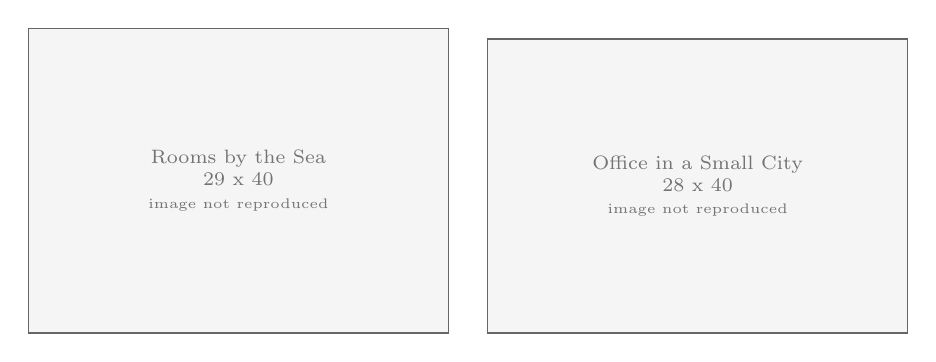
\begin{tikzpicture}
\draw[fill=black!4,draw=black!60,line width=0.5pt] (0,0) rectangle (5.333333333333333,3.8666666666666667);
\node[align=center,text=black!55,font=\scriptsize] at (2.6666666666666665,1.9333333333333333) {Rooms by the Sea\\29 x 40\\\tiny image not reproduced};
\draw[fill=black!4,draw=black!60,line width=0.5pt] (5.833333333333333,0) rectangle (11.166666666666666,3.7333333333333334);
\node[align=center,text=black!55,font=\scriptsize] at (8.5,1.8666666666666667) {Office in a Small City\\28 x 40\\\tiny image not reproduced};
\end{tikzpicture}
\caption{\textbf{Rooms by the Sea}, oil, September 1951; alias « The Jumping Off Place », 29 x 40 as the leaf writes it (Book III, leaf 41, ref 18347). Yale University Art Gallery, 1961.18.29: \url{https://lux.collections.yale.edu/view/object/63bdda22-a6be-413d-9a35-5e2649c14c21}. \textbf{Office in a Small City}, oil, September 1953, 28 x 40 as the leaf writes it (Book III, leaf 49, ref 18028). The Metropolitan Museum of Art, 53.183: \url{https://www.metmuseum.org/art/collection/search/488730}. Scale: sixty inches to eight centimetres; the two 28-by-40 and 29-by-40 formats of the studio pictures of 1949 to 1954. The frames are drawn to the proportions of the size in Edward Hopper's hand; the images are not reproduced here and can be seen at the museums' own pages. Drawn by Claude Fable~5.1, 13 September 2026, from the transcriptions and \texttt{works.json} (2026-09-13).}\label{fig:roomsoffice}
\end{figure}


\section{The buyers}

Book III names a buyer on every leaf, which Book IV, as we shall see, only begins to do in 1954. Stephen Clark is the collector of the volume: Rooms for Tourists in 1946, \q{Now owned by Griswold of Yale}; Rooms by the Sea in 1952, \q{snapped up at once before shown publicly}; Western Motel in 1958; Sunlight in a Cafeteria in 1958 at 9000; four Mexican and Wyoming watercolours besides. And then the note in pencil at the foot of Excursion into Philosophy:

\begin{leafquote}
On hearing about this canvas, Stephen Clark had come to see it. At old 5'' Ave. address, he learned of gallery moving to E. 64'' St., but when he got there, gallery locked, no one there. He wrote to tell us of his disappointment, but died a short time after that. It should have been his picture. \hfill (\lf{Book III}{69}{18472})
\end{leafquote}

\noindent Joseph Hirshhorn bought First Row Orchestra and 11 A.M. together for 5500 in September 1954, Hotel by a Railroad the same month and City Sunlight the year after; Lawrence Fleischman bought New York Office at 16,500 in January 1963 and \q{passed to Jos. Butler in exchange for an Eakins}; Howard Mack bought Intermission at 25,000; the Detroit museum Sun in an Empty Room at 25,000; the Whitney, through Lloyd Goodrich, Second Story Sunlight at 15,000 \q{less museum's 1/6} and the gallery's third, so that of fifteen thousand dollars the painter received 8333.34, in two cheques thirteen months apart. Museums appear as buyers and as juries: \q{During Retrospective at Whitney. Metrop. turned down this canvas for purchase.} (Conference at Night, \lf{Book III}{29}{17590}); \q{Note from Met to tell E. his Conference at Night has passed both juries} says the diary of November 1950, and Wichita bought it in 1952. The verso facing Morning in a City preserves a collector's doubt: \q{Stephen Clark wagging his head, predicted “You'll have a hard time disposing of this one.”} (ref 16404). It went to Lawrence Bloedel in 1955 for 6000, the highest price in the book to that date.

One sale went wrong, and the book follows it for eight years. Solitude, of 1944, was \q{Sold 1953 - Septm 4500 - to be paid weekly installments of 500. \unc{Chambers}? Caught up on litigation* \ldots\ Paid 500 down. \ldots\ Who has the picture? No news. Feb. 1958 + no further payments - than first 500.} The asterisk: \q{Caused by death of Frank Rehn + previous long illness}. And the end: \q{Rec'd July 3, 1961 - Acquired by lawyer Zacker who retained 2000 for him self. Stanley Wolf now owns, has paid up all charges} (\lf{Book III}{9}{17356}). The same passage records that \q{“Moonlight Interior” badly damaged found in an auction.} The dealer's illness of 1953 to 1956 runs under this volume like a fault line: payments \q{caught up in Rehn Estate}, October on Cape Cod paid only in June 1956 \q{by John Clancy, new head of Rehn Gallery}.

\begin{figure}[htbp]\centering
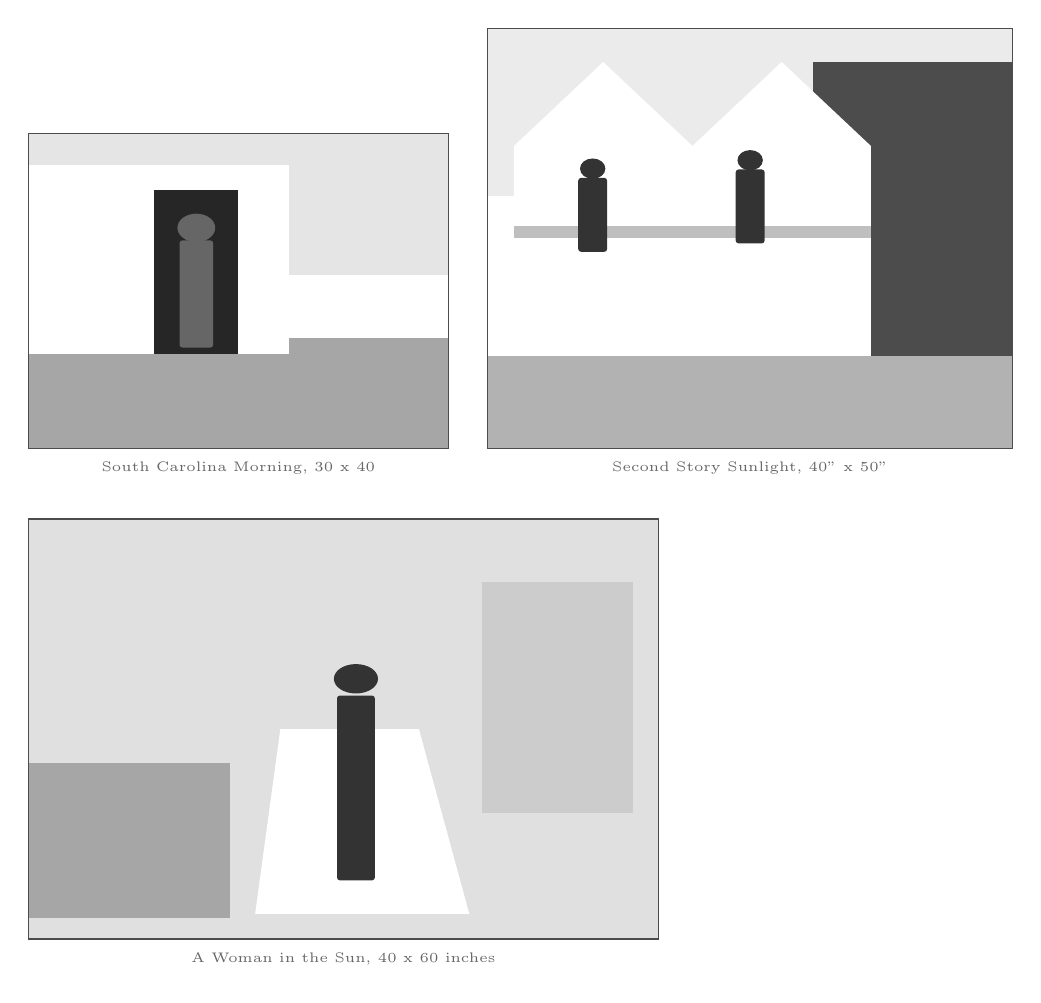
\begin{tikzpicture}
\begin{scope}[shift={(0,0)},x=5.333cm,y=4.000cm]\clip (0,0) rectangle (1,1);
\fill[black!10] (0,0.55) rectangle (1,1);           % sky
\fill[black!35] (0,0) rectangle (1,0.35);           % field
\fill[white] (0,0.3) rectangle (0.62,0.9);          % the house front
\fill[black!85] (0.3,0.3) rectangle (0.5,0.82);     % the doorway
\fill[black!60] (0.4,0.7) circle (0.045); \fill[black!60,rounded corners=1pt] (0.36,0.32) rectangle (0.44,0.66); % « Dinah »
\end{scope}
\draw[black!70,line width=0.5pt] (0,0) rectangle (5.333333333333333,4);
\node[anchor=north,font=\tiny,text=black!60] at (2.6666666666666665,-0.05) {South Carolina Morning, 30 x 40};
\begin{scope}[shift={(5.833333333333333,0)},x=6.667cm,y=5.333cm]\clip (0,0) rectangle (1,1);
\fill[black!8] (0,0.6) rectangle (1,1);             % sky
\fill[black!70] (0.62,0.2) rectangle (1,0.92);      % the woods behind
\fill[black!30] (0,0) rectangle (1,0.22);           % grass
\fill[white] (0.05,0.22) -- (0.05,0.72) -- (0.22,0.92) -- (0.39,0.72) -- (0.39,0.72) -- (0.56,0.92) -- (0.73,0.72) -- (0.73,0.22) -- cycle; % two gables
\fill[black!25] (0.05,0.5) rectangle (0.73,0.53);   % the balcony rail
\fill[black!80] (0.2,0.6659999999999999) circle (0.0242); \fill[black!80,rounded corners=1pt] (0.17250000000000001,0.46799999999999997) rectangle (0.2275,0.644); \fill[black!80] (0.5,0.6859999999999999) circle (0.0242); \fill[black!80,rounded corners=1pt] (0.4725,0.488) rectangle (0.5275,0.664);       % « Gothic + Elderly », « Toots »
\end{scope}
\draw[black!70,line width=0.5pt] (5.833333333333333,0) rectangle (12.5,5.333333333333333);
\node[anchor=north,font=\tiny,text=black!60] at (9.166666666666666,-0.05) {Second Story Sunlight, 40" x 50"};
\begin{scope}[shift={(0,-6.233333333333333)},x=8.000cm,y=5.333cm]\clip (0,0) rectangle (1,1);
\fill[black!12] (0,0) rectangle (1,1);
\fill[black!35] (0,0.05) rectangle (0.32,0.42);     % the bed
\fill[black!20] (0.72,0.3) rectangle (0.96,0.85);   % the window, landscape out of it
\fill[white] (0.36,0.06) -- (0.7,0.06) -- (0.62,0.5) -- (0.4,0.5) -- cycle; % « this Early light » on the floor
\fill[black!80] (0.52,0.62) circle (0.035); \fill[black!80,rounded corners=1pt] (0.49,0.14) rectangle (0.55,0.58); % the figure standing in it
\end{scope}
\draw[black!70,line width=0.5pt] (0,-6.233333333333333) rectangle (8,-0.9000000000000004);
\node[anchor=north,font=\tiny,text=black!60] at (4,-6.283333333333333) {A Woman in the Sun, 40 x 60 inches};
\end{tikzpicture}
\caption{\textbf{South Carolina Morning}, oil, 1955; « Dinah », 30 x 40 as the leaf writes it (Book III, leaf 53, ref 18558). Whitney Museum of American Art, 67.13: \url{https://whitney.org/collection/works/789}. \textbf{Second Story Sunlight}, oil, 25 August to 15 September 1960; « Toots », 40" x 50" as the leaf writes it (Book III, leaf 73, ref 17872). Whitney Museum of American Art, 60.54: \url{https://whitney.org/collection/works/873}. \textbf{A Woman in the Sun}, oil, October 1961; « the WISE TRAMP », 40 x 60 inches as the leaf writes it (Book III, leaf 75, ref 17107). Whitney Museum of American Art, 84.31: \url{https://whitney.org/collection/works/1337}. Scale: sixty inches to eight centimetres; the three formats of the last decade, 30 by 40, 40 by 50 and 40 by 60. The drawings are schemas of the composition in its main masses only, at the proportions of the size in Edward Hopper's hand, made from the leaf's description and from general knowledge of the picture; nothing is traced and no detail is drawn, and they are not reproductions. The pictures themselves are at the museums' own pages. Drawn by Claude Fable~5.1, 13 September 2026, from the transcriptions and \texttt{works.json} (2026-09-14).}\label{fig:late}
\end{figure}


\section{The prices}

The sale sentence is the same as Book II's, and the sequence it yields is the clearest statement of what happened to the market for Hopper's work in the last twenty years of his life. Hotel Lobby, 1943: 2500. Summer in the City, 1949: 1200, the lowest oil price in the book, to Lynn Farnol. High Noon and Conference at Night, 1951--52: 3000. Rooms by the Sea, 1952: 4000. Morning Sun, Hotel by a Railroad, First Row Orchestra, 1954: 3500. Sea Watchers, 1956: 4500. Hotel Window, 1957: 7000. Sunlight in a Cafeteria, 1958: 9000. November, Washington Square, 1960: 10,000. Excursion into Philosophy, 1962: 14,500. People in the Sun, 1962: 15,000. New York Office, 1963: 16,500. Sun in an Empty Room, 1964, and Intermission, 1966: 25,000. Chair Car, 1966: 27,000, paid in two instalments and never written in full. The painter's share was two thirds of each, and the last picture of all, The Two Comedians, \q{Finished Nov. 10'', 1966 in S. Truro studio}, has no buyer and no price (\lf{Book III}{89}{16659}).

The Memoranda leaves put the figures in a context she found bitter. \q{Light at 2 Lights sent with Exhib. of Amer. paintings to Russia, Summer 1959. On its return was sold for Richard Tucker by Lloyd Goodrich of the Whitney then to Laurence Fleishman, Collectors, for 25 000, top price for Amer. painting + nearly 25 times the amt. rec'd by the painter from his mother who bought it in 1929.} (\lf{Book III}{191}{16408}). The arithmetic in that sentence is hers, and it is the only resale price in the volume. The watercolours went the same way at a lower level: 600 and 750 in the 1940s, 900 in 1955, 1500 in 1960 and 1962, 1800 for Cliffs near Mitla in 1959, and 6500 for Charleston Slum, a sheet of 1929, in December 1964.

\begin{figure}[htbp]\centering
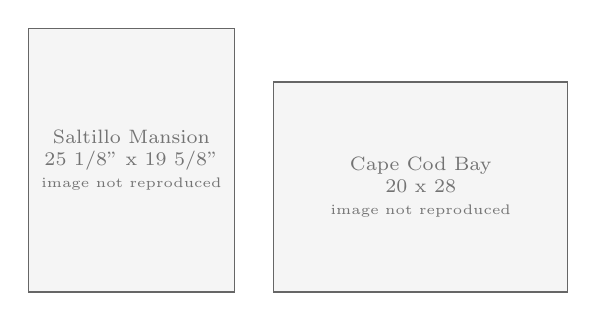
\begin{tikzpicture}
\draw[fill=black!4,draw=black!60,line width=0.5pt] (0,0) rectangle (2.6166666666666667,3.35);
\node[align=center,text=black!55,font=\scriptsize] at (1.3083333333333333,1.675) {Saltillo Mansion\\25 1/8" x 19 5/8"\\\tiny image not reproduced};
\draw[fill=black!4,draw=black!60,line width=0.5pt] (3.1166666666666667,0) rectangle (6.85,2.6666666666666665);
\node[align=center,text=black!55,font=\scriptsize] at (4.983333333333333,1.3333333333333333) {Cape Cod Bay\\20 x 28\\\tiny image not reproduced};
\end{tikzpicture}
\caption{\textbf{Saltillo Mansion}, watercolour, August 1943, 25 1/8" x 19 5/8" as the leaf writes it (Book III, leaf 101, ref 17944). The Metropolitan Museum of Art, 45.157.2: \url{https://www.metmuseum.org/art/collection/search/488165}. \textbf{Cape Cod Bay}, watercolour, 1965; the last work leaf photographed, 20 x 28 as the leaf writes it (Book III, leaf 125, ref 16620). Whitney Museum of American Art, work 6829: \url{https://whitney.org/collection/works/6829}. Scale: sixty inches to eight centimetres; an upright Mexican sheet of 1943 beside a Cape watercolour of 1965 on the full imperial sheet. The frames are drawn to the proportions of the size in Edward Hopper's hand; the images are not reproduced here and can be seen at the museums' own pages. Drawn by Claude Fable~5.1, 13 September 2026, from the transcriptions and \texttt{works.json} (2026-09-13).}\label{fig:watercolours}
\end{figure}


\section{Paint again}

The formula continues under nearly every oil, and Book III is where it can be followed year by year. Hotel Lobby, 1943: \q{W. + N. lead white. Blockx \& W. + N. Colors, linseed oil, turpentine. Winton canvas.} Morning in a City, 1944: \q{W. + N. flake white \# 1 + 2. Blockx + W. + N. colors. Tarr, Ruhl linseed oil + turpentine. Grumbacher's paint tested artists' canvas (linen).} The Martha McKeen: \q{Started with Tarr Ruhl linseed oil, finished with poppy oil}. From High Noon in 1949 to South Carolina Morning in 1955 the line is fixed: \q{Winsor \& Newton (National) double prime canvas and W \& N. colors, flake white, linseed oil and turpentine}, with Chremnitz white replacing flake from Morning Sun in 1952. From Sunlight on Brownstones in 1956 the canvas becomes \q{Herga}, single prime, and the transcription notices that \q{single} is struck out on four leaves and left on four others, and that \q{Nothing on any leaf says why}. The last formula, under The Two Comedians, is also the most explanatory: \q{W. + N. Herger Canvas, single white prime linen canvas + smoother as double would be, but less apt to crack than double. W. + N. lead white + Colors. Linseed oil with turpentine}. On High Noon a paler pencil adds: \q{E.H. made little model of house out of heavy white paper to observe how light would fall on corners of house.} (\lf{Book III}{31}{16818}). The diary of 31 August 1950 saw the \q{paper model for High Noon} on the desk.

\section{The end of the record}

The last picture leaf is dated 10 November 1966. The last money is Chair Car's balance on 16 December 1966, with \q{1967} in an unresolved line at the foot. The last date in the whole volume is \q{1967 Death of Arnold Slade of Truro} on a Memoranda leaf. Nothing in Josephine Hopper's hand records Edward Hopper's death on 15 May 1967, in any of the six books. The record was kept, as the inside cover of Book I said, \q{at time each work is finished, or before it leaves studio}, and when the work stopped so did the record.

The Memoranda also hold her account of the retrospective of 1950: \q{Hopper Retrospective in Boston - Canvases hung so closely frames nearly touched \ldots\ Very bad showing for oils.} and \q{At the Whitney, N.Y. - Everything glowed against beautiful walls} (\lf{Book III}{190}{17739}); of \emph{Reality}, \q{the first united squawk from the Realist painters against the usurpation of the Non objective people at the Mod. Mus., Whitney + many museums throughout the Country}; of the Time cover story of 1956, in the Reviews list, \q{E. Hopper Cover Story - (fraudulent + insulting)} (ref 17715); and of the Gold Medal of the Institute of Arts and Letters in 1955, in the Whereabouts: \q{Acceptance by E. H. not read by E. H. who only said “Thanks” until Henry P. shook him stoutly by shoulders + said “Say it again!”} (ref 17581). The Whereabouts leaf for 1960 records the house at last heated: \q{At 3 Wash. Sq. chaos with arrival of Hitler's aggressors, utter chaos, five studios turned into offices for Social Service Dept. But Radiators arrive for 1960 Xmas. So needn't go to Mexico to escape cold.} and \q{the enforced intimacy with almost affection + appreciation, an experience shared + the great reward: radiators} (\lf{Book III}{170}{18199}). Thirteen years after the Battle of Washington Square, the university that had tried to turn them out put in the heating.
